\documentclass[11pt,letterpaper]{article}
\usepackage[lmargin=1in,rmargin=1in,tmargin=1in,bmargin=1in]{geometry}
\usepackage{../style/homework}
\usepackage{../style/commands}
\setbool{quotetype}{true} % True: Side; False: Under
\setbool{hideans}{false} % Student: True; Instructor: False

% -------------------
% Content
% -------------------
\begin{document}

\homework{2: Due 02/10}{A book hasn't caused me this much trouble since Where's Waldo went to that barber pole factory.}{Tracy Jordan, 30 Rock}

% Problem 1
\problem{10} Represent each step in the following computation using fractions of a rectangle:
	\[
	\dfrac{2}{3} - \dfrac{1}{2}
	\] \pspace

\sol
	\[
	\begin{tikzpicture}
	\fill[gray!40] (0,0) -- (2,0) -- (2,1) -- (0,1);
	\draw[line width= 0.03cm] (0,0) -- (3,0) -- (3,1) -- (0,1) -- (0,0);
	\draw[line width= 0.03cm] (1,0) -- (1,1);
	\draw[line width= 0.03cm] (2,0) -- (2,1);
	\node at (1.5,-0.75) {$\dfrac{2}{3}$};
	
	\node at (4,0.5) {$-$};
	\node at (4,-0.65) {$-$};
	
	\fill[gray!40] (5,0) -- (6.5,0) -- (6.5,1) -- (5,1) -- (5,0);
	\draw[line width= 0.03cm] (5,0) -- (8,0) -- (8,1) -- (5,1) -- (5,0);
	\draw[line width= 0.03cm] (6.5,0) -- (6.5,1);
	\node at (6.5,-0.75) {$\dfrac{1}{2}$};
	\end{tikzpicture}
	\] \pspace

	\[
	\begin{tikzpicture}
	\fill[gray!40] (0,0) -- (2,0) -- (2,1) -- (0,1);
	\draw[line width= 0.03cm] (0,0) -- (3,0) -- (3,1) -- (0,1) -- (0,0);
	\draw[line width= 0.03cm] (1,0) -- (1,1);
	\draw[line width= 0.03cm] (2,0) -- (2,1);
	\draw[line width= 0.03cm] (0.5,0) -- (0.5,1);
	\draw[line width= 0.03cm] (1.5,0) -- (1.5,1);
	\draw[line width= 0.03cm] (2.5,0) -- (2.5,1);
	\node at (1.5,-0.75) {$\dfrac{4}{6}$};
	
	\node at (4,0.5) {$-$};
	\node at (4,-0.65) {$-$};
	
	\fill[gray!40] (5,0) -- (6.5,0) -- (6.5,1) -- (5,1) -- (5,0);
	\draw[line width= 0.03cm] (5,0) -- (8,0) -- (8,1) -- (5,1) -- (5,0);
	\draw[line width= 0.03cm] (5.5,0) -- (5.5,1);
	\draw[line width= 0.03cm](6,0) -- (6,1);
	\draw[line width= 0.03cm] (6.5,0) -- (6.5,1);
	\draw[line width= 0.03cm] (7,0) -- (7,1);
	\draw[line width= 0.03cm] (7.5,0) -- (7.5,1);
	\node at (6.5,-0.75) {$\dfrac{3}{6}$};
	\end{tikzpicture}
	\]

	\[
	\begin{tikzpicture}
	\fill[gray!40] (0,0) -- (0.5,0) -- (0.5,1) -- (0,1);
	\draw[line width= 0.03cm] (0,0) -- (3,0) -- (3,1) -- (0,1) -- (0,0);
	\draw[line width= 0.03cm] (1,0) -- (1,1);
	\draw[line width= 0.03cm] (2,0) -- (2,1);
	\draw[line width= 0.03cm] (0.5,0) -- (0.5,1);
	\draw[line width= 0.03cm] (1.5,0) -- (1.5,1);
	\draw[line width= 0.03cm] (2.5,0) -- (2.5,1);
	\node at (1.5,-0.75) {$\dfrac{1}{6}$};
	\end{tikzpicture}
	\]


\newpage



% Problem 2
\problem{10} Showing all your work, reduce the following rational numbers:
	\begin{enumerate}[(a)]
	\item $\dfrac{10}{14}$
	\item $\dfrac{18}{30}$
	\item $\dfrac{11}{17}$
	\item $\dfrac{36}{15}$
	\end{enumerate} \pspace

\sol
\begin{enumerate}[(a)]
\item 
	\[
	\dfrac{10}{14}= \dfrac{2 \cdot 5}{2 \cdot 7}= \dfrac{\cancel{2} \cdot 5}{\cancel{2} \cdot 7}= \dfrac{5}{7}
	\] \pspace

\item 
	\[
	\dfrac{18}{30}= \dfrac{2 \cdot 3^2}{2 \cdot 3 \cdot 5}= \dfrac{\cancel{2} \cdot 3^{\cancel{2}^1}}{\cancel{2} \cdot \cancel{3} \cdot 5}= \dfrac{3}{5}
	\] \pspace

\item 
	\[
	\dfrac{11}{17}= \dfrac{11}{17}
	\] \pspace

\item 
	\[
	\dfrac{36}{15}= \dfrac{2^2 \cdot 3^2}{3 \cdot 5}= \dfrac{2^2 \cdot 3^{\cancel{2}^1}}{\cancel{3} \cdot 5}= \dfrac{12}{5}
	\]
\end{enumerate}



\newpage



% Problem 3
\problem{10} Showing all your work and reducing as much as possible, perform the following computations: 
	\begin{enumerate}[(a)]
	\item $\dfrac{2}{3} - \dfrac{5}{7}$
	\item $\dfrac{5}{6} + \dfrac{7}{2}$
	\item $\dfrac{3}{4} - \dfrac{11}{6}$
	\item $\dfrac{1}{2} - \dfrac{1}{3} + \dfrac{3}{4}$
	\end{enumerate} \pspace

\sol
\begin{enumerate}[(a)]
\item 
	\[
	\dfrac{2}{3} - \dfrac{5}{7}= \dfrac{14}{21} - \dfrac{15}{21}= -\dfrac{1}{21}
	\] \pspace

\item 
	\[
	\dfrac{5}{6} + \dfrac{7}{2}= \dfrac{5}{6} + \dfrac{21}{6}= \dfrac{26}{6}= \dfrac{13}{3}
	\] \pspace

\item 
	\[
	\dfrac{3}{4} - \dfrac{11}{6}= \dfrac{9}{12} - \dfrac{22}{12}= -\dfrac{13}{12}
	\] \pspace

\item 
	\[
	\dfrac{1}{2} - \dfrac{1}{3} + \dfrac{3}{4}= \dfrac{6}{12} - \dfrac{4}{12} + \dfrac{9}{12}= \dfrac{11}{12}
	\]
\end{enumerate}



\newpage



% Problem 4
\problem{10} Showing all your work and reducing as much as possible, perform the following computations: 
	\begin{enumerate}[(a)]
	\item $\dfrac{7}{6} \cdot \dfrac{12}{3}$
	\item $-\dfrac{3}{4} \cdot \dfrac{12}{27}$
	\item $\dfrac{6}{35} \cdot \dfrac{14}{15}$
	\item $-\dfrac{10}{7} \cdot - \dfrac{5}{3}$
	\end{enumerate} \pspace

\sol
\begin{enumerate}[(a)]
\item 
	\[
	\dfrac{7}{6} \cdot \dfrac{12}{3}= \dfrac{7}{\cancel{6}} \cdot \dfrac{\cancel{12}^2}{3}= \dfrac{14}{3}
	\] \pspace

\item 
	\[
	-\dfrac{3}{4} \cdot \dfrac{12}{27}= -\dfrac{\cancel{3}}{\cancel{4}} \cdot \dfrac{\cancel{12}^{\cancel{3}^1}}{\cancel{27}^{\cancel{9}^1}}= -\dfrac{1}{3}
	\] \pspace

\item 
	\[
	\dfrac{6}{35} \cdot \dfrac{14}{15}= \dfrac{\cancel{6}^2}{\cancel{35}^5} \cdot \dfrac{\cancel{14}^2}{\cancel{15}^5}= \dfrac{4}{25}
	\] \pspace

\item 
	\[
	-\dfrac{10}{7} \cdot - \dfrac{5}{3}= \dfrac{50}{21}
	\]
\end{enumerate}



\newpage



% Problem 5
\problem{10} Showing all your work and reducing as much as possible, perform the following computations: 
	\begin{enumerate}[(a)]
	\item $\dfrac{\;\;\dfrac{4}{5}\;\;}{\;\;\dfrac{2}{15}\;\;}$
	\item $\dfrac{\;\;\dfrac{3}{4}\;\;}{\;\;\dfrac{5}{2}\;\;}$
	\item $\dfrac{\;\;\dfrac{3}{7}\;\;}{\;\;\dfrac{5}{6}\;\;}$
	\item $\dfrac{\;\;\dfrac{14}{33}\;\;}{\;\;\dfrac{10}{21}\;\;}$
	\end{enumerate} \pspace

\sol
\begin{enumerate}[(a)]
\item 
	\[
	\dfrac{\;\;\dfrac{4}{5}\;\;}{\;\;\dfrac{2}{15}\;\;}= \dfrac{4}{5} \cdot \dfrac{15}{2}= \dfrac{\cancel{4}^2}{\cancel{5}} \cdot \dfrac{\cancel{15}^3}{\cancel{2}}= 6
	\] \pspace

\item 
	\[
	\dfrac{\;\;\dfrac{3}{4}\;\;}{\;\;\dfrac{5}{2}\;\;}= \dfrac{3}{4} \cdot \dfrac{2}{5}= \dfrac{3}{\cancel{4}^2} \cdot \dfrac{\cancel{2}}{5}= \dfrac{3}{10}
	\] \pspace

\item 
	\[
	\dfrac{\;\;\dfrac{3}{7}\;\;}{\;\;\dfrac{5}{6}\;\;}= \dfrac{3}{7} \cdot \dfrac{6}{5}= \dfrac{18}{35}
	\] \pspace

\item 
	\[
	\dfrac{\;\;\dfrac{14}{33}\;\;}{\;\;\dfrac{10}{21}\;\;}= \dfrac{14}{33} \cdot \dfrac{21}{10}= \dfrac{\cancel{14}^7}{\cancel{33}^{11}} \cdot \dfrac{\cancel{21}^7}{\cancel{10}^5}= \dfrac{49}{55}
	\]
\end{enumerate}



\newpage



% Problem 6
\problem{10} Convert the following mixed fraction to an improper fraction:
	\[
	3\,\frac{4}{7}
	\]

\sol
	\[
	3\,\frac{4}{7}= \dfrac{3(7) + 4}{7}= \dfrac{21 + 4}{7}= \dfrac{25}{7}
	\]



\newpage



% Problem 7
\problem{10} Convert the following improper fraction to a mixed number:
	\[
	\dfrac{27}{5}
	\]

\sol
	\[
	\dfrac{27}{5}= \dfrac{25 + 2}{5}= \dfrac{25}{5} + \dfrac{2}{5}= 5 + \dfrac{2}{5}= 5\,\frac{2}{5}
	\]



\newpage



% Problem 8
\problem{10} Showing all your work, represent the following fractions as a decimal:
	\begin{enumerate}[(a)]
	\item $\dfrac{5}{8}$
	\item $\dfrac{4}{11}$
	\end{enumerate} \pspace

\sol
\begin{enumerate}[(a)]
\item 
	\[
	\longdivision{5}{8}
	\] \pspace
	\[
	\dfrac{5}{8}= 0.625
	\] \pspace

\item 
	\[
	\longdivision{4}{11}
	\] \pspace
	\[
	\dfrac{4}{11}= 0.\overline{36}
	\]
\end{enumerate}



\newpage



% Problem 9
\problem{10} Convert the following decimal to a fraction---reducing as much as possible:
	\[
	0.45
	\] \pspace

\sol
	\[
	0.45= \dfrac{45}{100}= \dfrac{3^2 \cdot \cancel{5}}{2^2 \cdot 5^{\cancel{2}^1}}= \dfrac{9}{20}
	\]



\newpage



% Problem 10
\problem{10} Convert the following decimal to a fraction---reducing as much as possible:
	\[
	0.636363\overline{63}
	\] \pspace

\sol \par
	\begin{table}[!ht]
	\centering\small
	\begin{tabular}{rccc}
	& $100N$ & $=$ & $63.636363\overline{63}$ \\ 
	$-$ & $N$ & $=$ & $\phantom{63.}0.63636363\overline{63}$ \\ \hline
	& $99N$ & $=$ & $63$ \\[0.1cm]
	& $N$ & $=$ & $\frac{63}{99}$ \\[0.1cm]
	& $N$ & $=$ & $\frac{7}{11}$
	\end{tabular}
	\end{table} \par

	\[
	0.\overline{63}= \dfrac{7}{11}
	\]


\end{document}